\capitulo{3}{Conceptos teóricos}

%En aquellos proyectos que necesiten para su comprensión y desarrollo de unos conceptos teóricos de una determinada materia o de un determinado dominio de conocimiento, debe existir un apartado que sintetice dichos conceptos.

\section{Medusas}
Las medusas son animales marinos formados por un cuerpo gelatinoso del que cuelga un manubrio tubular, encontrando la boca en la parte inferior de este. Algunas especies, tienen tentáculos con celular urticantes denominadas cnidocitos. Las medusas se desplazan mediante contracciones de su cuerpo absorbiendo agua para luego ser expulsada de manera brusca provocando el movimiento~\cite{wiki:medusas}.

Su reproducción es asexual, siendo esta, una fecundación externa mediante óvulos y espermatozoides que son liberados por los machos y las hembras respectivamente. Esto da lugar a la fecundación de gametos que se convertirán en larvas denominadas plánulas. Más adelante estas larvas se adhieren a alguna superficie donde se transformarán en pólipos para finalmente desprenderse la medusa adulta~\cite{noauthor_reproduccion_2016}.


\begin{figure}%[!h]
	\centering
	\includegraphics[width=0.9\textwidth]{reproducciónMedusas.jpg}
	\caption[Fases del proceso de reproducción de las medusas]{Fases del proceso de reproducción de las medusas~\cite{reproduccionMedusas}.}
	\label{fases_medusas}
\end{figure}


Su alimentación se basa principalmente en plancton aunque también son capaces de comer crustáceos, huevos o peces pequeños.

En este caso, la especie que estamos estudiando se trata de la \emph{Physalia physalis}, también conocida como la fragata portuguesa. Esta no es realmente una medusa, sino que es un organismo colonial formado por varios tipos de hidroides o individuos pólipo (Figura \ref{esquema_carabela}) y pertenece a la clase de los Hydrozoos. A pesar de esto, su comportamiento y reproducción es igual al de las medusas por lo que las trataremos como tal.
Consta de un flotador lleno de gas para mantener la flotabilidad y que tiene forma de vela para facilitar su desplazamientos por el viento~\cite{physalia}.

\begin{figure}%[!h]
	\centering
	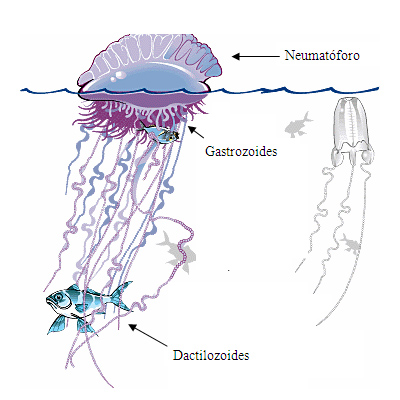
\includegraphics[width=0.9\textwidth]{carabela.jpg}
	\caption[Partes del cuerpo de una fragata portuguesa]{Partes del cuerpo de una fragata portuguesa~\cite{esquema-carabela}.}
	\label{esquema_carabela}
\end{figure}

\subsection{Comportamiento de las medusas}
Los colonias de medusas están muy influenciadas por las condiciones climatológicas y marítimas. La temperatura, salinidad, el viento y las corrientes son los principales factores a tener en cuenta.

El peso de estos factores en los desplazamientos de las colonias varía en función de la etapa de desarrollo en la que se encuentren. Las que tienen un tamaño pequeño o mediano, están más condicionadas a la dirección de los vientos y las corrientes ya que, debido a su pequeño tamaño, no son capaces de contrarrestar estas fuerzas. Por otro lado, en las medusas de un tamaño superior, estos factores tienen menos relevancia mientras que la salinidad del agua y la temperatura de la misma adquieren un mayor protagonismo.Por ejemplo, hasta unos 25 grados, \texttt{}el numero de medusas va en aumento. A partir de ese punto, la concentración de las mismas decrece.

\textit{\say{La reproducción de estas también se ve influenciada por la temperatura del agua pues según diferentes experimentos se ha demostrado que existe una relación entre el aumento de las temperaturas y una mayor reproducción asexual en varias especies gelatinosas}}~\cite{canepa_environmental_2017}. 

Los factores humanos también tienen su influencia en los movimientos de las poblaciones de medusas y en su reproducción. 
El aumento de materia orgánica provocado por vertidos como podrían ser los de una EDAR (Estación Depuradora de Aguas Residuales) o de una explotación agrícola, que provoca la eutrofización del medio haciendo que las medusas puedan desarrollarse de una manera más rápida. Del mismo modo, la construcción de estructuras costeras, proporcionan lugares donde pueden proliferar con mayor facilidad.

Teniendo en cuenta todo esto, diferentes estudios concluyen que estas alteraciones aleatorias del medio, tiene poca influencia en el desarrollo de las colonias de medusas, mientras que las condiciones ambientales que se repiten anualmente tiene una mayor importancia en comparación. Esto remarca la importancia de un análisis de las condiciones ambientales que provocan estos brotes para poder anticiparse a ellos~\cite{art:ArticuloCanepa_1}.

\section{Knowledge Discovery in Databases (KDD)}

Actualmente se recopila una gran cantidad de información de todos los ámbitos y es necesario darla un uso práctico. La \textbf{minería de datos} es un campo de las ciencias de la computación por el cual se tratan de descubrir nuevos patrones o relaciones en conjuntos de datos de manera automática. Con estas nuevas relaciones se trata de explicar comportamientos actuales o predecir resultados futuros~ \cite{mineria_tecnicas_herramientas}. 

Sin embargo, la minería de datos es solo una fase del proceso de descubrimiento del conocimiento (KDD). El \emph{Knowledge Discovery} se trata de la búsqueda de conocimiento en los datos. Su objetivo es la extracción de información útil y previamente desconocida de conjuntos de datos. Estos los podemos obtener de multitud de formas diferentes por lo que es necesario un proceso de preparación de los mismos.

Posteriormente, es cuando podremos utilizar algoritmos de clasificación o regresión para lograr un modelo resultante en forma de reglas o patrones, que siendo interpretados, obtendremos nuevo conocimiento.

Un resumen de todo el proceso del KDD se puede observar en la Figura~\ref{fasesKDD}.

\begin{figure}%[!h]
	\centering
	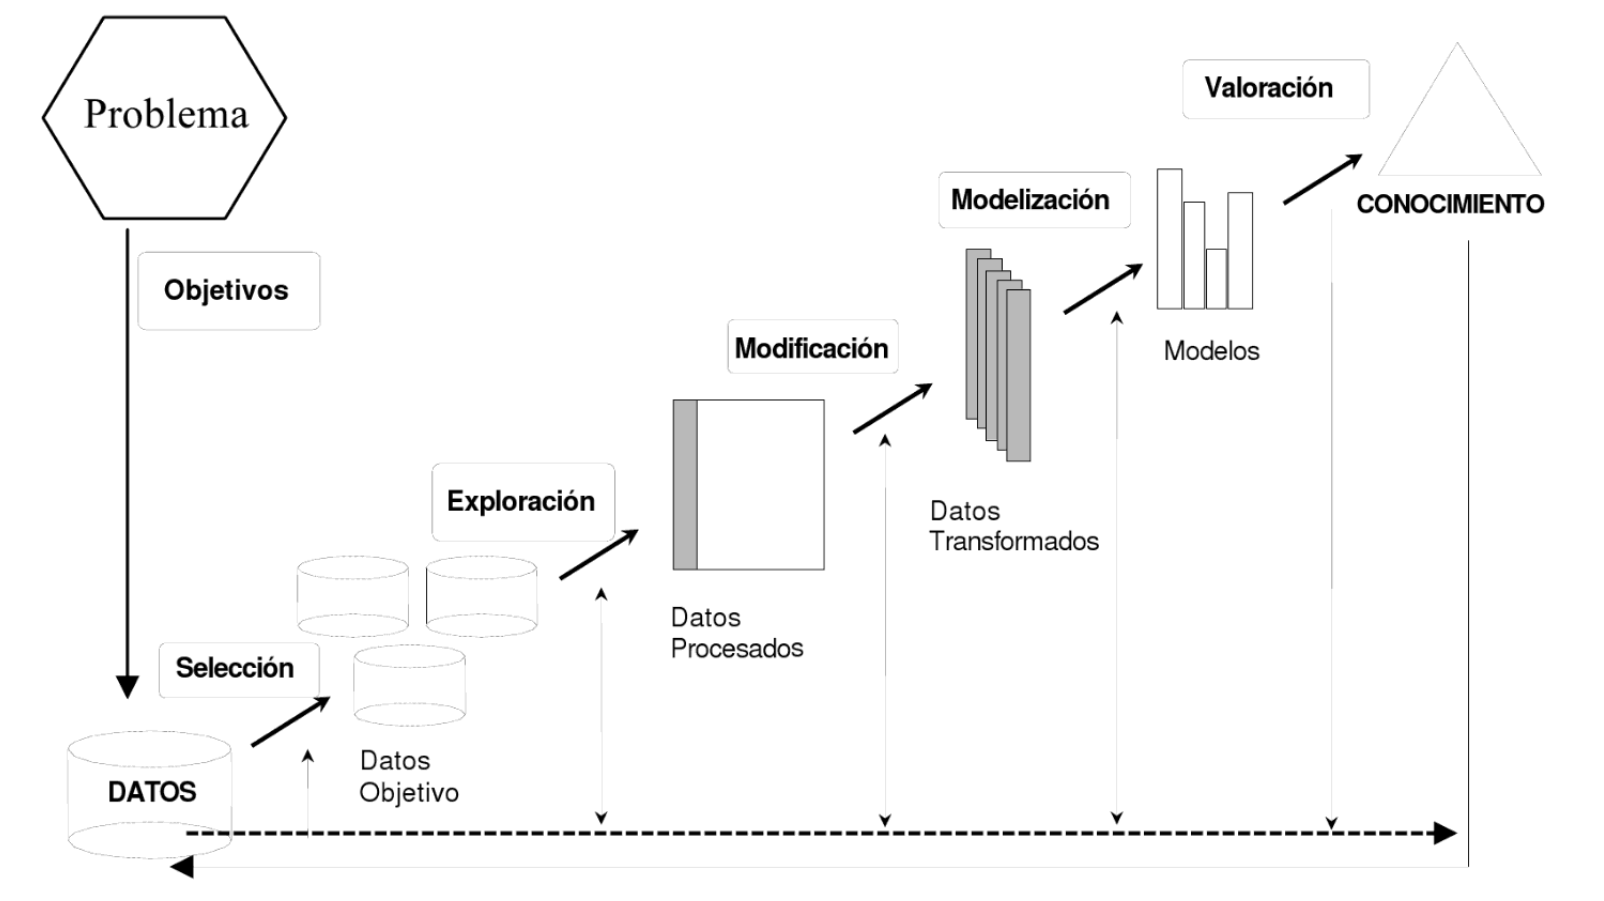
\includegraphics[width=0.9\textwidth]{esquemaMineria.png}
	\caption[Fases del proceso de KDD]{Fases del proceso de KDD~\cite{mineria_tecnicas_herramientas}.}
	\label{fasesKDD}
\end{figure}

\textcolor{green}{Añadir subsección de la obtención de los datos}
\subsection{Preprocesamiento de los datos}
Se trata del primer paso una vez obtenido el conjunto de datos a utilizar. Estos datos en bruto no pueden ser utilizados en los algoritmos de minería sin un tratamiento previo. El conjunto de datos inicial debe ser transformado a un formato estándar para poder ser analizado.

Una vez conseguido, no se puede asumir que la información que contiene sea válida o correcta. Pueden existir variables que introduzcan ruido en la muestra o campos que se hayan introducido de manera errónea. También puede ocurrir que no se necesite la totalidad de la información contenida en el dataSet, sino que unicamente se requiera parte de la misma. Como ocurre en este caso, solo es de interés la el área geográfica de Chile y el área de los océanos cercana a sus costas.

Otro problema que se encuentra, son los valores nulos o la falta de los mismos. Ya sea por fallos es el grabado de la información o falta de la misma, es necesario corregir esos valores vacíos pudiendo descartar esas instancias o reemplazarlas por otros valores razonables teniendo en cuenta su contexto~\cite{libro_mineria}.

Finalmente se pueden aplicar al conjunto otras técnicas como la normalización de los datos.

\subsection{Minería de datos}
Como se ha comentado anteriormente, la minería de datos se trata de obtener patrones o relaciones a partir de conjuntos de datos.

En nuestro caso, se pretende conseguir un modelo capaz de encontrar relaciones entre el estado de la mar y la aparición de medusas en la costa. Para ello el modelo debe ser capaz de aprender a partir de los datos de entrada. Se pueden definir dos tipos de aprendizaje principales: supervisado y no supervisado.

\subsubsection{Aprendizaje supervisado}
Se trata de modelo que se elaboran a partir de conjuntos de datos etiquetados, es decir cada instancia tiene un atributo que es el valor a predecir. Este atributo será una clase ([mucho/poco], [alto/bajo]...) si se trata de un problema de clasificación, mientras que si se trata de un problema de regresión será un valor numérico.

Una vez entrenado el modelo, éste podrá etiquetar o predecir el valor de para nuevas instancias.
En este caso tenemos un problema de regresión pues se intenta entrenar un modelo que prediga el número de avistamientos de medusas.

\subsubsection{Aprendizaje no supervisado}
En este caso, el entrenamiento del modelo no se hace con datos etiquetados sino que se les asignan características. A partir de los datos de entrada, se agrupa a los datos en conjuntos en función de estas características. Estos grupos se denominan \emph{clusters} de instancias.

\subsubsection{Series temporales}
Las series temporales son sucesiones de datos que han sido tomados o medidos  secuencialmente a lo largo del tiempo~\cite{SeriesTempUBU}.
Estas tienen una serie de características:
\begin{itemize}
	\item El valor medido o magnitud.
	\item La periodicidad, se trata de la repetición en el tiempo de los valores de manera cíclica.
	\item La tendencia es la variación que se observa en la media de los valores a largo plazo.
	\item El ruido que son valores aleatorios sin explicación.
\end{itemize}

Con estos componentes, podríamos separa una serie en sus diferentes partes (Figura \ref{descomposicion_series}).

\begin{figure}%[!h]
	\centering
	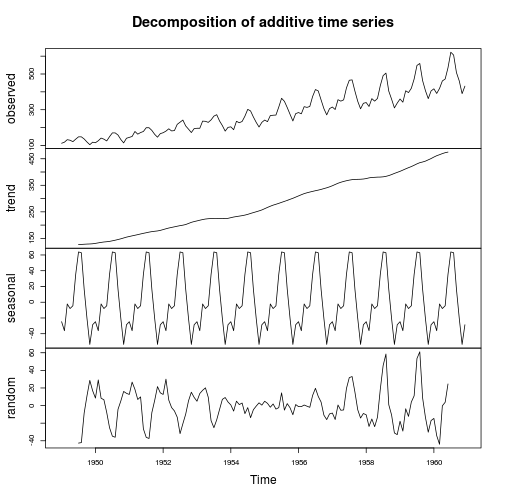
\includegraphics[width=0.9\textwidth]{descomposicion_series.png}
	\caption[Descomposición de una serie temporal]{Descomposición de una serie temporal~\cite{SeriesTemp}.}\label{descomposicion_series}
\end{figure}

Las series temporales pueden ser regulares o irregulares, es decir, serán regulares cuando la separación (distancia temporal) entre las diferentes medidas es constante, mientras que la irregulares esta separación es variable.

Un punto importante es el de la estacionariedad. Una serie temporal puede ser estacionaria cuando su media y varianza se mantienen constantes con el paso del tiempo, es decir, no dependen de este y ademas no presentan tendencia. Por otro lado, en una serie no estacionaria, estos valores si cambian a lo largo del tiempo pudiendo encontrar variaciones de tendencia, varianza o co-varianza.

Tres ejemplos de esto podrían ser los reflejados en la figura \ref{series_no_estacionarias}.

\begin{figure}%[!h]
	\centering
	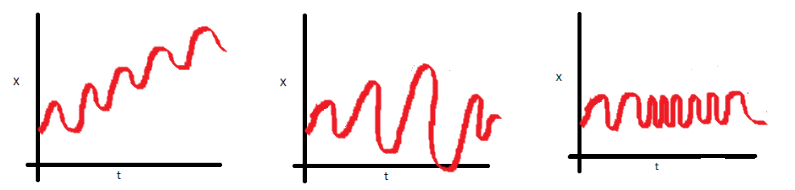
\includegraphics[width=0.9\textwidth]{estacionariedad_no.png}
	\caption[Ejemplo de series temporales no estacionarias]{Ejemplo de series temporales no estacionarias~\cite{SeriesTempIMG}.}\label{series_no_estacionarias}
\end{figure}

\begin{itemize}
	\item En el primer gráfico podemos observar como la media aumenta con el transcurso del tiempo, esto provoca una tendencia creciente, por lo que estamos frente a una serie no estacionaria.
	\item En el segundo caso la varianza de la serie no es constante por lo que tampoco es una serie estacionaria.
	\item Por último caso, la co-varianza varía en función del tiempo por lo que no es una serie estacionaria. 
\end{itemize}

\begin{figure}%[!h]
	\centering
	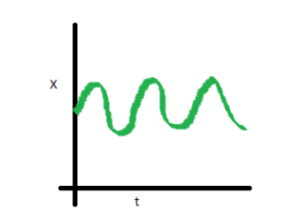
\includegraphics[width=0.6\textwidth]{estacionariedad_si.png}
	\caption[Ejemplo de serie temporal estacionaria]{Ejemplo de serie temporal estacionaria~\cite{SeriesTempIMG}.}\label{serie_si_estacionaria}
\end{figure}

En el caso de la figura \ref{serie_si_estacionaria}, encontramos una serie con media, varianza y co-varianza constante por lo que si que podríamos hablar de una serie estacionaria. 

\subsection{Evaluación del modelo}



%Algunos conceptos teóricos de \LaTeX \footnote{Créditos a los proyectos de Álvaro López Cantero: Configurador de Presupuestos y Roberto Izquierdo Amo: PLQuiz}.
%
%
%
%\section{Secciones}
%
%Las secciones se incluyen con el comando section.
%
%\subsection{Subsecciones}
%
%Además de secciones tenemos subsecciones.
%
%\subsubsection{Subsubsecciones}
%
%Y subsecciones. 
%
%
%\section{Referencias}
%
%Las referencias se incluyen en el texto usando cite \cite{wiki:latex}. Para citar webs, artículos o libros \cite{koza92}.
%
%
%\section{Imágenes}
%
%Se pueden incluir imágenes con los comandos standard de \LaTeX, pero esta plantilla dispone de comandos propios como por ejemplo el siguiente:
%
%\imagen{escudoInfor}{Autómata para una expresión vacía}
%
%
%
%\section{Listas de items}
%
%Existen tres posibilidades:
%
%\begin{itemize}
%	\item primer item.
%	\item segundo item.
%\end{itemize}
%
%\begin{enumerate}
%	\item primer item.
%	\item segundo item.
%\end{enumerate}
%
%\begin{description}
%	\item[Primer item] más información sobre el primer item.
%	\item[Segundo item] más información sobre el segundo item.
%\end{description}
%	
%\begin{itemize}
%\item 
%\end{itemize}
%
%\section{Tablas}
%
%Igualmente se pueden usar los comandos específicos de \LaTeX o bien usar alguno de los comandos de la plantilla.
%
%\tablaSmall{Herramientas y tecnologías utilizadas en cada parte del proyecto}{l c c c c}{herramientasportipodeuso}
%{ \multicolumn{1}{l}{Herramientas} & App AngularJS & API REST & BD & Memoria \\}{ 
%HTML5 & X & & &\\
%CSS3 & X & & &\\
%BOOTSTRAP & X & & &\\
%JavaScript & X & & &\\
%AngularJS & X & & &\\
%Bower & X & & &\\
%PHP & & X & &\\
%Karma + Jasmine & X & & &\\
%Slim framework & & X & &\\
%Idiorm & & X & &\\
%Composer & & X & &\\
%JSON & X & X & &\\
%PhpStorm & X & X & &\\
%MySQL & & & X &\\
%PhpMyAdmin & & & X &\\
%Git + BitBucket & X & X & X & X\\
%Mik\TeX{} & & & & X\\
%\TeX{}Maker & & & & X\\
%Astah & & & & X\\
%Balsamiq Mockups & X & & &\\
%VersionOne & X & X & X & X\\
%} 
